\documentclass[10pt]{article}

\usepackage[T1]{fontenc}
\usepackage[utf8]{inputenc}
%\usepackage{beton}
%\usepackage{ccfonts}
%\usepackage{concrete}
\usepackage{concmath}
\usepackage{eulervm}
\usepackage{amsmath,amsthm,amssymb}
\usepackage{mathtools}
\usepackage{multicol}
\usepackage{marginnote}
\usepackage{pgfplots}
\usepackage{float}
\usepackage{hyperref}
\usepackage{bbm}
\usepackage{booktabs}
\pgfplotsset{compat=1.5}

\usepackage{listings}
\usepackage{xcolor}
\definecolor{codegreen}{rgb}{0,0.6,0}
\definecolor{codegray}{rgb}{0.5,0.5,0.5}
\definecolor{codepurple}{rgb}{0.58,0,0.82}
\definecolor{backcolour}{rgb}{0.95,0.95,0.92}
\lstdefinestyle{mystyle}{
    backgroundcolor=\color{backcolour},   
    commentstyle=\color{codegreen},
    keywordstyle=\color{magenta},
    numberstyle=\tiny\color{codegray},
    stringstyle=\color{codepurple},
    basicstyle=\ttfamily\footnotesize,
    breakatwhitespace=false,         
    breaklines=true,                 
    captionpos=b,                    
    keepspaces=true,                 
    numbers=left,                    
    numbersep=5pt,                  
    showspaces=false,                
    showstringspaces=false,
    showtabs=false,                  
    tabsize=2
}

\lstset{language=Python, style=mystyle}

\usepackage{mathtools}

\usepackage{wasysym}
\usepackage[margin=1.5in]{geometry} 
\usepackage{enumerate}
\index{\usepackage}\usepackage{multicol}

\newcommand{\N}{\mathbf{N}}
\newcommand{\Z}{\mathbb{Z}}

\newcommand{\R}{\mathbf{R}}
\newcommand{\C}{\mathbf{C}}
\newcommand{\Pbb}{\mathbb{P}}
\newcommand{\Fcal}{\mathcal{F}}
\newcommand{\Lcal}{\mathcal{L}}
\newcommand{\Acal}{\mathcal{A}}
\newcommand{\Ecal}{\mathcal{E}}
\newcommand{\Ebb}{\mathbb{E}}
\newcommand{\Qbb}{\mathbb{Q}}


\renewcommand{\mathbf}{\mathbold}

\newenvironment{theorem}[2][Theorem]{\begin{trivlist}
  \item[\hskip \labelsep {\bfseries #1}\hskip \labelsep {\bfseries #2.}]}{\end{trivlist}}
\newenvironment{lemma}[2][Lemma]{\begin{trivlist}
  \item[\hskip \labelsep {\bfseries #1}\hskip \labelsep {\bfseries #2.}]}{\end{trivlist}}
\newenvironment{exercise}[2][Exercise]{\begin{trivlist}
  \item[\hskip \labelsep {\bfseries #1}\hskip \labelsep {\bfseries #2.}]}{\end{trivlist}}
\newenvironment{reflection}[2][Reflection]{\begin{trivlist}
  \item[\hskip \labelsep {\bfseries #1}\hskip \labelsep {\bfseries #2.}]}{\end{trivlist}}
\newenvironment{proposition}[2][Proposition]{\begin{trivlist}
  \item[\hskip \labelsep {\bfseries #1}\hskip \labelsep {\bfseries #2.}]}{\end{trivlist}}
\newenvironment{corollary}[2][Corollary]{\begin{trivlist}
  \item[\hskip \labelsep {\bfseries #1}\hskip \labelsep {\bfseries #2.}]}{\end{trivlist}}

\newenvironment{definition}[2][Definition]{\begin{trivlist}
  \item[\hskip \labelsep {\bfseries #1}\hskip \labelsep {\bfseries #2.}]}{\end{trivlist}}

\begin{document}
	
  \renewcommand{\qedsymbol}{\smiley}
	\title{Investments Class \\ Problem set 4}
	\author{Daniel Grosu, William Martin, Denis Stiffen}
		
\maketitle

\begin{exercise}{1}(Risk Decomposition)
      A readout of the standard deviation of error between
      \textrm{03/17/08} and \textrm{03/14/11}, daily adjusted, figures up to
      $1.420\%$. To transform that into annualized units of variance, we perform
      the following computation:

      \begin{align*}
        var\left[ \epsilon \right] = \Delta^{-1} \sigma_{\Delta}^2 = 252 \times (1,420 \%)^2 = 508,13 \%^2.
      \end{align*}
      Where $252$ is the number of trading days in one year.
      The above error term is the volatility after controlling for market
      returns, hence it is the so-called idiosyncratic or diversifiable risk
      which in percentage units is

      \begin{align*}
        v_i = \sqrt{var\left[ \epsilon \right]} = 22,54 \%
      \end{align*}

      The raw beta of the Philip Morris International US Equity is $\beta =
      0.635$. The digest of statistical numbers in the sidebar does not contain
      the variance of the market return, but we can compute it by combining the
      $R^2$ and the $\beta$ statistics:

      \begin{align*}
        R^2 &= \frac{\beta_i^2 \sigma_M^2}{\beta_i^2 \sigma_M^2 + v_i^2} \\
        \sigma_M^2 &= \frac{R^2 v_i^2}{(1 - R^2) \beta_i^2} \\
        \sigma_M &= \sqrt{\frac{R^2}{(1 - R^2)}}\frac{v_i}{\beta_i} \\
        \sigma_M &= \sqrt{\frac{0.416}{1 - 0.416}} \frac{22.54\%}{0.635} = 29,96\%
      \end{align*}

      The systematic risk then is:
      \begin{align*}
        \beta_i^2 \sigma_M^2 = (0.635)^2(29,96\%)^2 = 361,93\%^2 = (19,02\%)^2
      \end{align*}

      The total risk $var\left[ R \right]$ is the sum of the systematic and the
      idiosyncratic risk:
      \begin{align*}
        var\left[ R \right] = \beta_i^2 \sigma_M^2 + var\left[ \epsilon \right] = (19,02\%)^2 + (22,54\%)^2 = (29,49\%)^2
      \end{align*}
\end{exercise}

\newpage

\begin{exercise}{2}

	After downloading the daily returns on the Amazon stock from CRSP, the CRSP value-weighted market return, and the short-term t-bill from 2009 to 2019, we plot our results
	
	\begin{figure}[H]
	
		\centering
		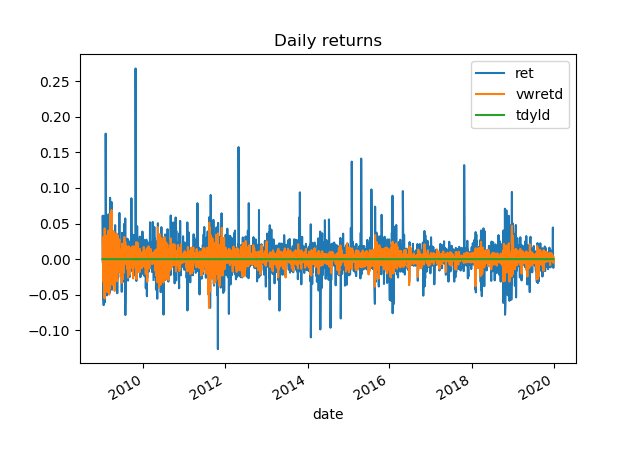
\includegraphics[scale=0.8]{figures/ex2_1.png}	
		\caption{Daily returns for 10 years of the Amazon stock (ret), the CRSP value-weighted  market return (vwretd) and the short-term t-bill (tdyld)}	
		\label{fig:ex2_1}	
	
	\end{figure} 
	
 	Before continuing our analysis, we compute the excess returns using the t-bill rate as the risk-free rate. We then compute the covariance matrix of these excess returns which gives us
	
	\begin{align*}
		\begin{pmatrix}
			0.000447 & 0.000117\\
			0.000117 & 0.000107
		\end{pmatrix}			
	\end{align*}	 
	
	Where the first element of the diagonal represents the variance of the excess returns on the Amazon stock and the second element of the diagonal the variance of the excess returns on the CRSP value-weighted market return. The non-diagonal elements are simply the covariance elements of the 2 aforementioned quantities. 	
	
	\smallbreak
	
	Computing the beta becomes straightforward
	
	\begin{align*}
		\beta = \frac{Cov(R, R_{M})}{Var(R_{M})} = 1.091364
	\end{align*}

	We now plot the rolling-window estimate of the beta of the stock using six month data-window. We also plot the adjusted beta series using the Bloomberg formula 
	
	\begin{align*}
		\beta_{adj} = w \times \beta_{est} + (1 - w) \times \beta_{avg}
	\end{align*}
	
	Where $\beta_{avg} = 1 $ and $w = 2/3$. We also plot the constant beta found above.
	
	\begin{figure}[H]
	
		\centering
		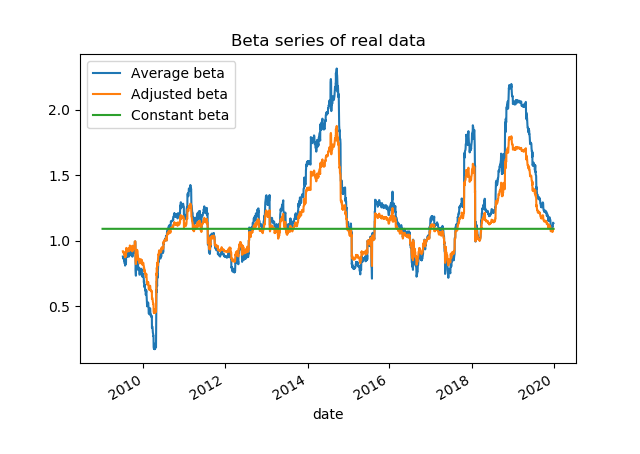
\includegraphics[scale=0.8]{figures/ex2_2.png}	
		\caption{Beta series of rolling-window estimate of beta, adjusted beta and constant beta using real data}	
		\label{fig:ex2_2}
				
	\end{figure}	

	We now simulated 10 years of data of excess returns for a stock that satisfies the CAPM equation. Using the formula below, we are able to compute idiosyncratic risk of the stock
	
	\begin{align*}
		Var(\epsilon) = Var(R) - \beta^{2} Var(R_{M})
	\end{align*}
	
	Below is the plot of the rolling-window estimate for the beta using simulated data this time (together with the adjusted and constant beta series)
	
	\begin{figure}[H]
	
		\centering
		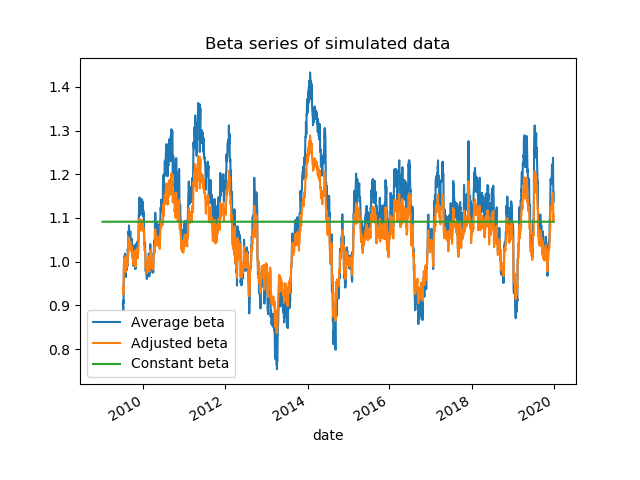
\includegraphics[scale=0.8]{figures/ex2_3.png}	
		\caption{Beta series of rolling-window estimate of beta, adjusted beta and constant beta using simulated data}
		\label{fig:ex2_3}
				
	\end{figure}
		
\end{exercise}

\newpage

\begin{exercise}{3}
  \begin{enumerate}[(a)]
    \item
      \textbf{FALSE.} The CAPM implies exactly the opposite: that all the stocks
      are represented by points on the security market line. The security market
      line being a bijection between returns and betas, it implies in particular
      that two securities of equal expected returns have the same beta.
    \item
      \textbf{FALSE.} Idiosyncratic risks do not matter at all for the CAPM
      because it is diversifiable. An investor may choose to invest in the
      security with higher idiosyncratic risk because its systematic risk
      (measured by beta) is smaller.

    \item
      \textbf{FALSE.} According to CAPM, standard deviation is the right measure
      of risk only for assets perfectly correlated with the market. Otherwise,
      the beta is the right measure of risk.
    \item
      The asset with positive alpha is currently undervalued. By no means should
      a mean-variance investor put all his wealth into this asset: in this way
      none of its idiosyncratic risk is diversified away.
      \item
        Yes. If the CAPM holds then the idiosyncratic risks must necessarily be
        uncorrelated. This owes to the fact that if some of the idiosyncratic
        risks are correlated then not all of it can be diversified away and
        there would be some risk premium which is not captured by beta. Another
        way to look at it is to interpret the idiosyncratic risk as the error term in the
        regression of the risky asset excess return on the market excess return which,
        under CAPM, is a true model and the error terms are homoskedastic hence uncorrelated.
  \end{enumerate}
\end{exercise}

\newpage

\begin{exercise}{4} 
	
\begin{itemize} 
	\item We know that the optimal portfolio when holding the riskless asset is given by: $$ w = \frac{1}{a}\Sigma^{-1}(\mu-R_0\mathbbm{1})$$
	And with the given values, we find the following weights in the mean-variance portfolio: $$ w_0 = (0.4846,0.3724,0.2978)$$ The sum of the three weights equals $1.1548$, so the investor borrows $0.1548$ at the risk-free rate to invest in the risky portfolio. 
	\item As all investors are mean-variance investors, they should invest in the optimal portfolio given in the previous point, with their respective risk aversion parameter $a$. We can use the relation given in the lecture to find the market portfolio: 
	$$w_0 = \frac{B-AR_0}{a}w_{tan}$$ and we also know that the tangency portfolio equals the market portfolio. This leads to the market weights: 
	$$ w_M = (0.4196, 0.3225, 0.2579)$$
	So the market return is $R_M = w_M'\mu = 9.68\%$ and the standard deviation of returns is $\sigma_M = \sqrt{w_M'\Sigma w_M} = 9.00\%$.
	\item A mean-variance investor will only invest in the market portfolio if the optimal portfolio is the same as the tangency portfolio (and thus the market one). So we require the condition $w_0 = w_{tan}$ that is equivalent with the previous equation to: $a_M = B-AR_0$. Thus, the economy-wide aggregate risk aversion is $a_M = 5.7742$. 
	\\
	So the implicit risk-aversion implied by the market portfolio is higher than the risk-aversion of investor X ($a=5$). This is consistent since X is borrowing at the risk-free rate whereas holders of the market portfolio do not lend or borrow on the riskless asset. Therefore, the economy-wide risk-aversion is expected to be higher. 
	\item Since the risk-free asset is in net zero supply, this means that if X borrows money at rate $R_0$, he can only achieve it with investor Y. There is no bank. So investor Y has to lend money to X at rate $R_0$. His position in the riskless asset is $-0.1548$ because they have the same initial wealth.  
	\item The optimal portfolio is given by the mean-variance optimal weights with no risk-free asset, but with the constraint $w'\mathbbm{1} = 1 - 0.1548 = 0.8452$ as Y has to lend this amount to X and it is required that they have the same initial wealth (the weights sum to $1$ with the risk-free weight).
	The optimal portfolio for investor Y should then satisfy the constraint: $w_Y'\mathbbm{1} = 0.8452$. 
	
	This is equivalent with $\mathbbm{1}'(\frac{1}{a_Y}\Sigma^{-1}(\mu-R_0\mathbbm{1}))= 0.8425$ and it is solved by $a_Y = 6.8317$. So this risk-aversion is much higher than the one of X because Y is lending in the riskless asset. 

	Finally, the optimal portfolio for investor Y is $$w_Y = \frac{1}{a_Y}\Sigma^{-1}(\mu-R_0\mathbbm{1}) = (0.3546, 0.2726, 0.2180)$$

\end{itemize}
\end{exercise}
  
\end{document}
